%%
%% Author: Philipp Tornow; Vanessa
%% 17.10.2018
%%

% Preamble
\documentclass[11pt]{article}

% Packages
\usepackage{amsfonts}
\usepackage{amsmath}
\usepackage{amsthm}
\usepackage{booktabs}
\usepackage{hyperref}
\usepackage{xspace}
\usepackage[utf8]{inputenc}
\usepackage{fancyvrb}
\usepackage{graphicx}
\usepackage{amssymb}
\usepackage[T1]{fontenc}
\usepackage{qtree}
\usepackage{multicol}

%Theorems
\newtheorem{thm}{Theorem}[section]
\newtheorem{cor}[thm]{Corollary}
\newtheorem{lem}[thm]{Lemma}
\newtheorem{prop}[thm]{Proposition}
\theoremstyle{definition}
\newtheorem{defn}[thm]{Definition}
\theoremstyle{remark}
\newtheorem{rem}[thm]{Remark}

% Document
\begin{document}

    \title{1. Übungsblatt\\
    Formale Sprachen (WiSe 18/2019)\\
    \textit{Bauhaus-Universität\ Weimar\\}
    }
    \author{Vanessa Retz\\
    \vspace{5mm}
    \normalsize Mat.Nr.:117380\\
    \large Philipp Tornow\\
    \vspace {5mm}
    \normalsize Mat.Nr.: 118332\\
    }

    \maketitle

    \newpage
    \section*{Aufgabe 1:}
    \subsection*{1.}
    \begin{normalsize}
        G(V,T,P,S)\\
        V = {S,A,B,C,D}\\
        T = {0,1}\\

        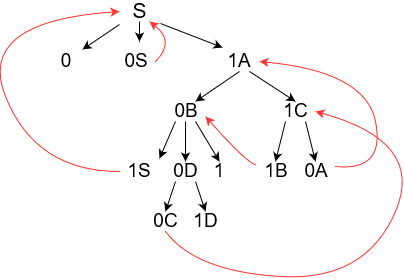
\includegraphics[width=0.8\textwidth]{Aufgabe1_1.png}

        \noindent
        Produktionsbeispiele:\\
        \begin{multicols}{2}

            \noindent
            0\\
            00\\
            000 \hspace{15mm} Rest: 0\\
            ... \\

            \noindent
            0\\
            0101 \rightarrow 5\\
            0101101 \rightarrow 45 \hspace{10mm} Rest: 0\\
            011001 \rightarrow 25\\

        \end{multicols}
        Bei dem Betrachten der Produktion aller Binärwörter der Sprache L(G) fällt auf, dass
        sobald eine Null angehangen wird, sich der Wert verdoppelt und wir wissen, dass wenn ein Wort
        durch 5 teilbar ist, das Doppelte (der doppelte Wert) ebenfalls durch 5 teilbar ist.
        Alternativ kann ein Wort der Sprache auch auf Eins (Verdopplung+1) terminieren, jedoch muss hierbei nach den
        Produktionsregeln eine 0 vorausgehen (0B). \\
        \vspace{10mm}
        IA: für Wortlänge 1 -> terminiert bei 0 \rightarrow \hspace{2mm} $0\mod5=0$\\
        IV: alle Worte beliebiger Wortlänge(n+1) befinden sich in der selben Restklasse\\
        IS: (noch nicht fertig)
    \end{normalsize}

    \subsection*{2.}
    \begin{normalsize}
         -> Aus A1 gilt, dass nur Binärzahlen/Worte terminieren, die mod 5=0 ergeben.\\
         -> In jedem Schritt kann eine 1 oder eine 0, also alle Elemente unseres Alphabets,
            hinzugefügt werden.\\
            Daraus folgt, dass alle Binärzahlen darstellbar sind, mit der Einschränkung Nichtterminalen am Ende stehen zu haben.\\
            Aus unserer Bedingung aus A1 wissen wir, dass nur Worte mod 5=0 terminieren und ein gültiges Wort bilden.\\
            Also sind alle binären Zeichenketten, welche als Binärzahl interpretiert eine durch 5 teilbare Zahl darstellen, in unserer Sprache L(G).
    \end{normalsize}

    \newpage
    \section*{Aufgabe 2:}
    \subsection*{1.}
    \begin{normalsize}
    	
    	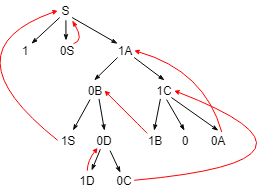
\includegraphics[width=0.8\textwidth]{Baum1.png}
    	\noindent
    	\\
    	\\
    	Um die Terminalsymbole zu bestimmen reicht es aus, sich ein Produktionsbeispiel anzusehen und bei den erforderlichen Stellen das Symbol einzusetzen welches noch benötigt wird um zu terminieren. \\
    	\\
    	Produktionsbeispiel:\\
    	\\
    	S $\rightarrow$ 0S (R = 0) $\rightarrow$ 01A (R = 1) $\rightarrow$ 010B (R = 2) $\rightarrow$ 0101S (R = 0) $\rightarrow$ $0101t_0$ mit $t_0 = 1$ ergibt $01011$ welches $11\mod5=1$ ergibt. \\
    	Nachdem $t_0$ nun 1 ist, kann $t_1$ nur noch 0 werden da aus dem Bereich der Terminalsymbole nurnoch die 0 übrig bleibt. \\
    	
    	$\rightarrow$ $\hspace{5mm}$ $t_0$ = 1 ; $\hspace{10mm}$ $t_1$ = 0 ;
    \end{normalsize}
    \subsection*{2.}
    \begin{normalsize}
    	
    	Um nun $\mod$ 5 den Rest 2 zu erhalten muss die Grammatik dementsprechend aus dem vorher akzeptierten Zustand verändert werden. 
    	Das vorherige Produktionsbeispiel kann folgendermaßen abgeändert werden : \\
    	\\
    	S $\rightarrow$ 0S (R = 0) $\rightarrow$ 01A (R = 1) $\rightarrow$ 010B (R = 2) $\rightarrow$ 0101S (R = 0) $\rightarrow$ 01011A (R = 1) \\
    	Wenn wir nun $t_1 = 0$ auf A verschieben bekommt man $010110$ was $22\mod5$ einen Rest von 2 ergibt. \\
    	Da $t_1$ nun auf A verschoben wurde, setzen wir $t_0$ auf C an die Stelle an welcher vorher $t_1$ war.  \\ 
    	Führen wir mit dieser Grammatik nun das Beispiel weiter, erhält man : \\
    	01011A (R = 1) $\rightarrow$ 010111C (R = 3) $\rightarrow$ 010111$t_0$ mit $t_0 = 1$ erhält man $0101111$ was $47\mod5 = 2$ entspricht (als Dezimalzahl interpretiert). \\
    	\\
    	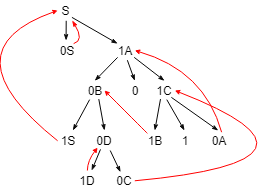
\includegraphics[width=0.8\textwidth]{Baum2.png}
    	\\
    	Um die Grammatik also abzuändern müssen die Reste nach den einzelnen Ableitungsschritten betrachtet werden und diejenigen welche man noch benötigt um terminieren zu können berücksichtigt werden. \\
    
    \end{normalsize}
\end{document}